\chapter{Estado del arte}
En este capítulo se hablará sobre el contexto en el que se enmarca este proyecto.

En primer lugar, se hará una breve explicación de como las herramientas open-source ayudan a agilizar el desarrollo y la funcionalidad en una red de telecomunicaciones.

Por último, se hace especial mención a los dos paradigmas que motivan este proyecto: SDN y NFV.

\section{Herramientas Open-Source en redes de telecomunicación}

Una red de telecomunicación es un conjunto de medios, tecnologías y protocolos que tienen como finalidad el intercambio de información entre diferentes usuarios.

Así mismo, se está produciendo una enorme evolución en el concepto de una red de telecomunicación. 

Antes, este concepto era puramente físico, con un conjunto de dispositivos \textit{Hardware}, como pueden ser \textit{routers}, \textit{switches} u ordenadores, interactuando entre sí. Actualmente, prácticamente el 100\% de las redes utilizan software open-source para diferentes propósitos:

\begin{itemize}
	\item Sacar máximo rendimiento a su infraestructura.
	\item Agilizar el envío y procesamiento del tráfico de la red.
	\item Acelerar y automatizar la gestión y configuración de los dispositivos.
	\item Reducir los costes de operación.
\end{itemize}

\subsection{Ejemplos}

Para conseguir los propósitos mencionados anteriormente, existen numerosas herramientas de software desarrolladas por empresas, universidades u organizaciones que están totalmente disponibles para ser usadas por cualquier usuario.

Algunas de estas herramientas son las siguientes:

\begin{itemize}
	\item \textbf{Docker:} Esta herramienta consiste en un proyecto de código abierto que automatiza el despliegue de aplicaciones dentro de contenedores de software, proporcionando una abstracción y automatización adicionales en múltiples sistemas operativos.
	
	\item \textbf{OpenStack:} 
\end{itemize}



\section{SDN}
\label{sec:sdn}

\begin{figure}[!ht]
	\centering
	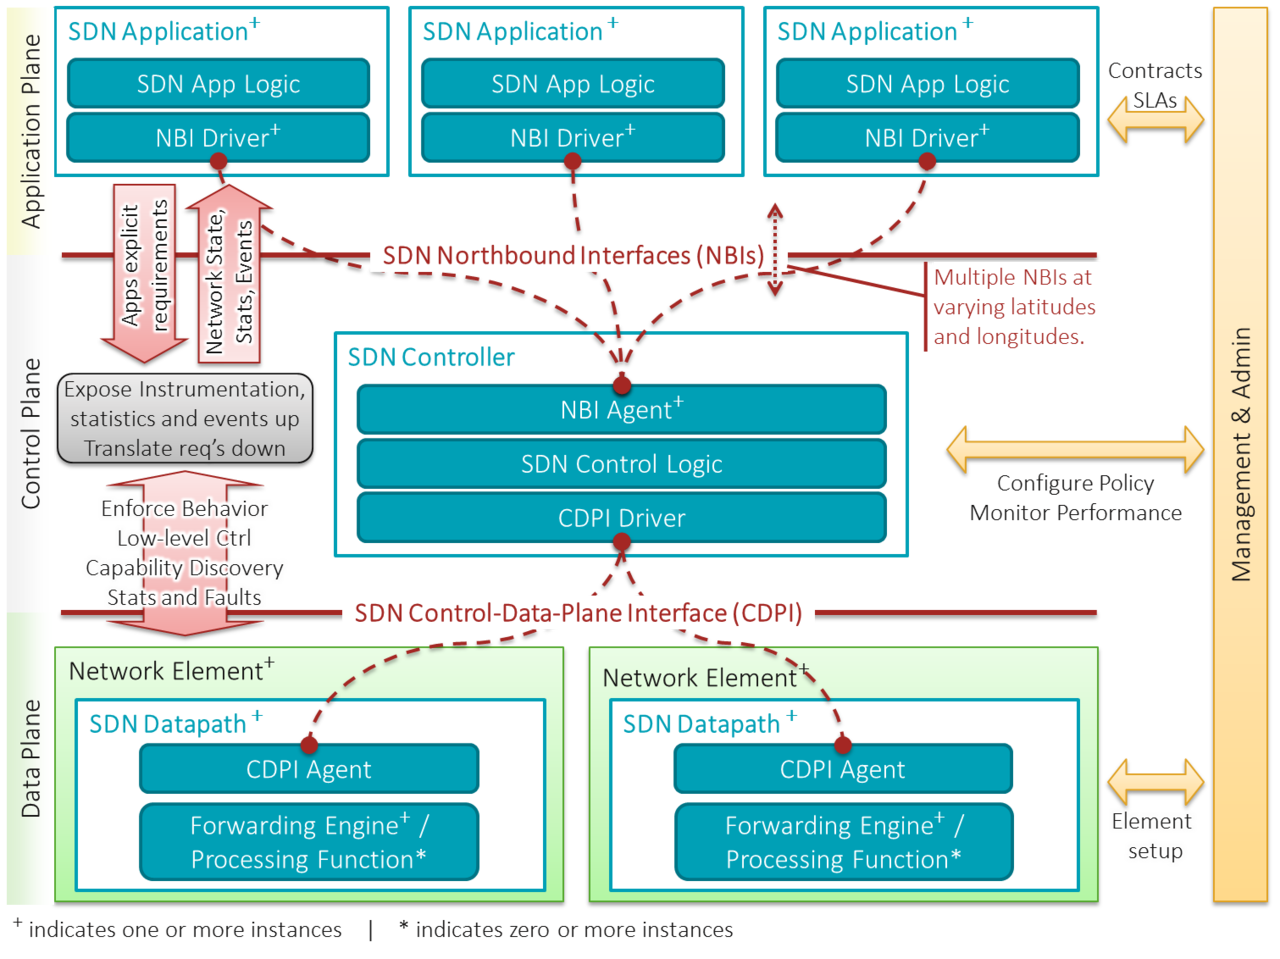
\includegraphics[width=0.75\linewidth]{imagenes/arquitectura_sdn}
	\caption{Arquitectura SDN}
	\label{fig:arquitecturasdn}
\end{figure}


\subsection{OpenFlow}
\label{subsec:openflow}

\section{NFV}
\label{sec:nfv}


\cleardoublepage